\documentclass{report}
\usepackage[T1]{fontenc} % Fontes T1
\usepackage[utf8]{inputenc} % Input UTF8
\usepackage[backend=biber, style=ieee]{biblatex} % para usar bibliografia
\usepackage{csquotes}
\usepackage[portuguese]{babel} %Usar língua portuguesa
\usepackage{blindtext} % Gerar texto automaticamente
\usepackage[printonlyused]{acronym}
\usepackage{hyperref} % para autoref
\usepackage{graphicx}
\usepackage{indentfirst}
\usepackage{comment}
\usepackage{float} % para forcar a imagem a ficar onde quero
\addbibresource{bibliografia.bib} % para indicar que o ficheiro de bibliografia é o bibliografia.bib

\begin{document}
%%
% Definições
%
\def\titulo{A evolução das espécies: Teoria e evidências}
\def\data{12/11/2024}
\def\autores{Gabriel Guzman, Henrique Tardelli}
\def\autorescontactos{(126180) getarache@ua.pt, (125087) henrique.tardelli@ua.pt}
\def\versao{VERSAO : 0.1.1}
\def\departamento{Dept. de Eletrónica, Telecomunicações e Informática}
\def\empresa{Universidade de Aveiro}
\def\logotipo{imagens/ua.pdf}
\def\repo{infor2024-ap-g18}
%
%%%%%% CAPA %%%%%%
%
\begin{titlepage}

\begin{center}
%
\vspace*{50mm}
%
{\Huge \titulo}\\ 
%
\vspace{10mm}
%
{\Large \empresa}\\
%
\vspace{10mm}
%
{\LARGE \autores}\\ 
%
\vspace{30mm}
%
\begin{figure}[h]
\center
\includegraphics{\logotipo}
\end{figure}
%
\vspace{30mm}
\end{center}
%
\begin{flushright}
\versao
\end{flushright}
\end{titlepage}

%%  Página de Título %%
\title{%
{\Huge\textbf{\titulo}}\\
{\Large \departamento\\ \empresa}
}
%
\author{%
    \autores \\
    \autorescontactos
}
%
\date{\today}
%
\maketitle

\pagenumbering{roman}


%%%%%% RESUMO %%%%%%
\begin{abstract}

O trabalho aborda a mudança e evolução dos seres vivos, cuja ideia foi introduzida no século XIX pelo grande cientista Charles Darwin. A teoria da evolução é a ideia de que as diferentes espécies evoluem ao longo de milhões de anos para a forma atual. A evolução ocorre porque os seres vivos em uma população que têm características que lhes permitem sobreviver e reproduzir são mais comuns. O ensaio proposto visa mesclar os fundamentos clássicos de Darwin com abordagens modernas que em muito ampliam e enriquecem a quebra de como tipos de seres vivos absolutamente não idênticos mudam ao longo de milhões de anos e adaptam-se. Os cientistas encontraram evidências, que aqui explicaremos e mostraremos, de que vários animais e plantas mudaram e adaptaram-se durante longos períodos através do estudo de ossos antigos e outros vestígios. Através dos fósseis, por exemplo, é possível observar as mudanças nas espécies ao longo de milhões de anos, fornecendo uma linha do tempo da evolução. Fósseis não só ajudam a entender como os organismos se transformaram, mas também fornecem pistas sobre os ambientes em que viveram. Ensinará também como a vasta gama de seres vivos na Terra não é apenas uma mistura aleatória, mas segue um padrão razoável e natural de como mudam ao longo do tempo. Portanto, a análise dos fósseis é essencial para compreender a evolução e a história da vida no nosso planeta.


\end{abstract}

%%%%%% Agradecimentos %%%%%%
% Segundo glisc deveria aparecer após conclusão...
%\renewcommand{\abstractname}{Agradecimentos}
%\begin{abstract}
%Eventuais agradecimentos.
%Comentar bloco caso não existam agradecimentos a fazer.
%\end{abstract}

\renewcommand{\contentsname}{Índice}
\tableofcontents
% \listoftables     % descomentar se necessário
% \listoffigures    % descomentar se necessário


%%%%%%%%%%%%%%%%%%%%%%%%%%%%%%%
\clearpage
\pagenumbering{arabic}

%%%%%%%%%%%%%%%%%%%%%%%%%%%%%%%%
\chapter{Introdução}
\label{chap.introducao}

Uma expedição científica ao longo das margens da América do Sul, no século XIX, tornou-se uma aventura de descobertas sobre a vida. Durante a viagem, Darwin ficou impressionado com a diversidade de formas de vida que testemunhou e começou a formular sua abordagem da origem das espécies e do processo pelo qual as mudanças biológicas são provocadas.
Por unanimidade, o tema foi escolhido pelas suas características interessantes, relevantes e atemporais, segundo os membros conformantes do grupo: é um dos maiores marcos da história e da ciência num todo, mudou a forma com que nós autopercebemos, assim como também a forma que vemos nossas origens e de todos os outros animais no mundo. 
Presentamos uma análise/resenha da \textit{Teoria da Evolução}. Depois desta introdução, no \autoref{chap.fundamentos} são apresentados os príncipios nos quais baseia-se a teoria, em seguida no \autoref{chap.Genetica} são explicados os conceitos da teoria num paradigma que envolve os estudos realizados a finais do século XX, incluindo genética e mutações como pontos mais importantes, a seguir no \autoref{chap.Evidencias} referem-se as provas físicas e mais evidentes que sustentam a teoria, por último no \autoref{chap.Evolucao} são mostradas as aplicações da teoria em espécies contemporâneas. 

\chapter{Fundamentos da Teoria da Evolução}\label{chap.fundamentos}

Neste capítulo, vamos a explorar as bases da teoria baseadas no Darwinismo clássico \cite{darwin.origin.2008}, entender como ela surgiu e por que é tão importante para compreender a vida na Terra. Veremos em que se baseia e como ajuda a explicar a diversidade de organismos e as conexões indivíduo-ambiente.

\section{A variabilidade intraespecífica}\label{sec.variacao}

No Darwinismo clássico a \textbf{variabilidade intraespecífica} entre os indivíduos de uma população era fundamental, pois ela fornecia a \textit{matéria-prima} sobre a qual a seleção natural atuaria. Essas diferenças nas características dos indivíduos não eram vistas por Darwin como sendo criadas por um mecanismo explícito, mas sim como variações \textit{espontâneas} que surgiam em uma população. 

\section{Seleção natural}\label{sec.selecaon}

A seleção natural é um dos principais mecanismos de evolução propostos por Charles Darwin em "A Origem das Espécies" \cite{darwin.origin.2008}. O processo natural ocorre quando indivíduos dentro de uma população possuem variações nas suas características \autoref{sec.variacao} (como tamanho, cor, resistência a doenças), e algumas dessas variações oferecem uma vantagem de sobrevivência e reprodução em determinado ambiente. Indivíduos com características vantajosas têm maior probabilidade de sobreviver, se reproduzir e transmitir essas características para as próximas gerações. Ao longo de muitas gerações resulta em mudanças significativas nas populações, levando à adaptação das espécies ao ambiente. Um exemplo clássico da seleção natural ocurreu nas \textbf{ilhas Galápagos}, onde Darwin observou que as espécies de tentilhões variavam em tamanho e forma do bico, como se pode observar a figura\ref{fig:tenti}. 

\begin{figure}[h]
\center
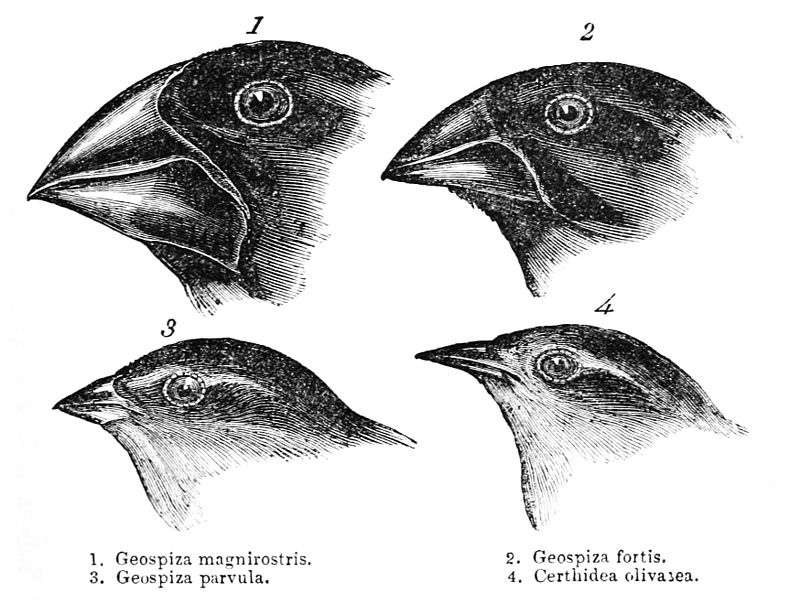
\includegraphics[width=0.7\textwidth]{imagens/darwinfinches.jpg}
\caption{Tentilhões de Darwin}
\label{fig:tenti}
\end{figure}

\subsection{Principios da seleção natural}

\begin{enumerate}

  \item \textbf{Luta pela sorevivência} :Os recursos, como alimento, espaço e parceiros reprodutivos, são limitados, gerando competição entre os indivíduos, por exemplo num espaço com pouca água as plantas competem pela pouca quantidade disponível.
  
  \item \textbf{Sobrevivência dos mais aptos} :Apenas indivíduos com características que conferem vantagens específicas no ambiente (como a capacidade de lutar, escapar de predadores ou resistir a doenças), terão mais chances de sobreviver até a maturidade e se reproduzir, transmitindo essas características para seus descendentes.
  
  \item \textbf{Acúmulo gradual de características favoráveis} :A união sequencial de características ventajosas (por gerações) de varios indivíduos, ocasionará que os descendentes estejam melhor adaptados e dotados de múltiples características favoravéis. Destacando que em ocasiôes os individuos podem não possuir características adaptativas ao ambiente, mas sim características que \textit{facilitam} sua reprodução.

\end{enumerate}

\section{Seleção sexual}

Por vezes, as características associadas com a sobrevivência e adaptação não são as que garantem a preservação de uma espécie, mas sim as ligadas com a atração sexual de fémeas. Esta \textit{luta} não acaba com a morte do contediente mais fraco, mas com a redução do número dos seus descendentes (ou a inexistência dos mesmos). A selecção sexual é por isso menos rigorosa que a selecção natural. Na natureza ocorre nos chifres dos veados, o esporão dos galos, as cores vivas nas aves pequenas, danças e cantos em outras espécies de aves. 

\section{Leis da variação}

As leis da variação propostas por Charles Darwin são princípios que explicam como as diferenças entre indivíduos de uma espécie surgem e como essas diferenças alimentam o processo evolutivo. Darwin declarou: "\textit{As alterações estruturais, tão complexas e inumeráveis, que podemos observar em toda a natureza, não podem ter sido todas simplesmente causadas por este tipo de acção.}", ou seja, a seleção natural possui maior relevância, porém deve agir em simultaneidade com as leis da variação.
  
\subsection{Efeito do uso ou desuso de partes}

O uso ou desuso de orgãos e partes do corpo continuado ao longo de gerações da mesma espécie, refletem uma mudança na descendencia, seja desenvolvendo os músculos associados, ou atrofiando-os. Aclarando que este conceito deve entender-se como um subordinado da seleção natural, se o uso ou desuso for beneficioso para a sobrevivência da espécie uma mudança ocorrerá. Exemplificando: se a cauda de um rato for cortada seu descendente obviamente nascera com uma cauda normal, pois as mudanças não são inmediatas nem arbitrárias. 

\subsection{Aclimatação}

É extremamente comum encontrarmos espécies do mesmo género a habitar em países quentes e em países
frios. Se considerarmos que todas as espécies de um género derivam de uma mesma forma parental, temos de supor que as espécies tiveram de passar por um processo de aclimatação ao longo das gerações. A adaptação de cada espécie ao clima do meio em que vive é evidente: as espécies do árctico, ou mesmo de um clima temperado,não conseguem aguentar um clima tropical, e vice-versa. 

\subsection{Isolamento geográfico}

Numa área confinada, ou isolada, desde que não seja muito grande, as condições de vida, orgânicas e inorgânicas, são geralmente uniformes em todo o território. Assim, a selecção natural tenderá a modificar todos os indivíduos variáveis de uma espécie da mesma maneira. Nestas áreas, por estarem fechadas, o cruzamento com os habitantes dos territórios vizinhos é impossível. O isolamento permite que uma variedade nova se aperfeiçoe lentamente, como mostrado na imagem \ref{fig:isolamento} , sem constrangimentos temporais.


\begin{figure}[h] %el H mayuscula, forzo la imagen a quedar en el lugar deseado.
\center
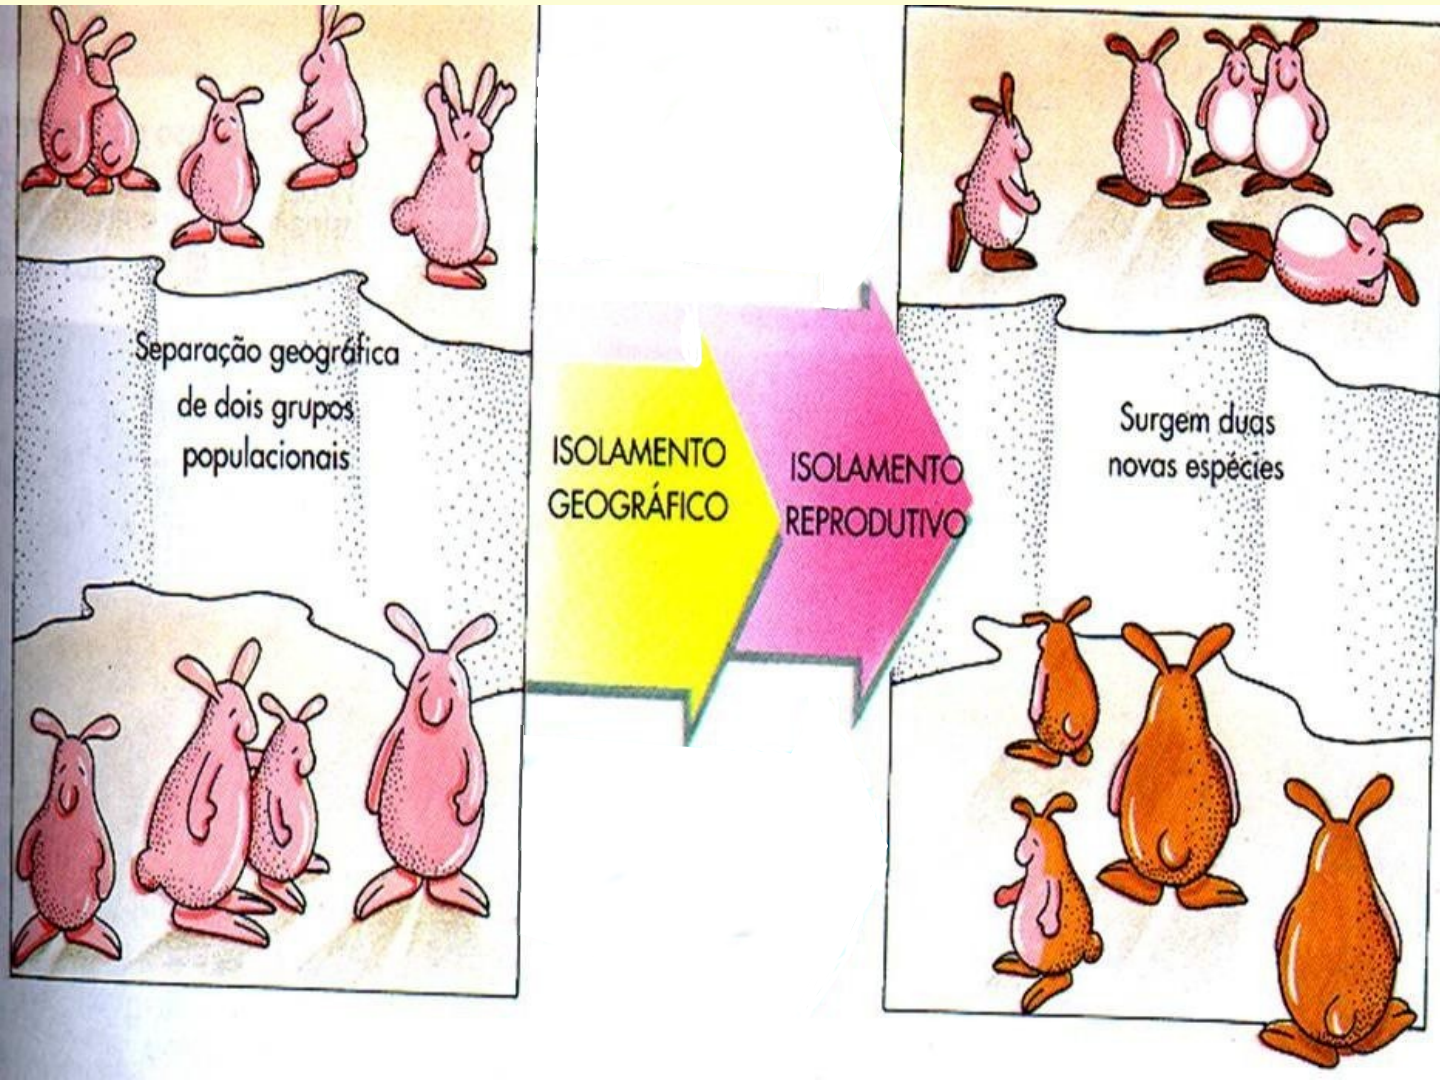
\includegraphics[width=0.6\textwidth]{imagens/isolamento2.png}
\caption{Processo de isolamento geográfico}
\label{fig:isolamento}
\end{figure}


\section{Divergência e convergência de caracteres}

Na divergência seres vivos que, aparentemente, são diferentes podem apresentar semelhanças anatómicas, orgãos homólogos, que podem sugerir a existência de um ancestral comum, com um plano estrutural idêntico aos seus ascendentes. que por divisão territorial ou mudança do ambiente adaptaram-se a outro meio. \\

Por outro lado na convergência seres vivos de diferentes espécies sem um ancestro comun, desenvolvem orgãos análogos, adaptados ao ambiente onde habitam. Pode-se observar uma descrição mais gráfica de este conceito na imagem \ref{fig:gencia} .Deste tema fala-se mais adiante e de maneira mais aprofundada \ref{sec.fosseis2}. \\

\begin{figure}[h] 
\center
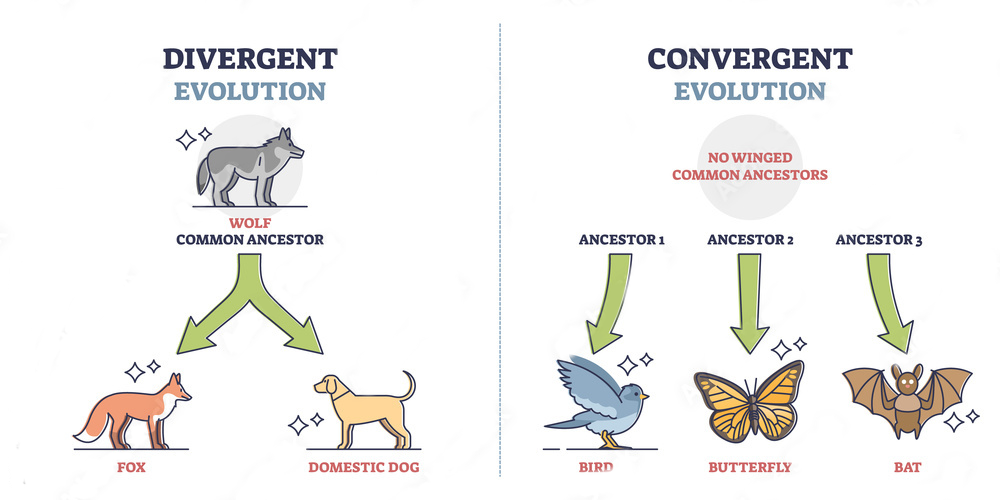
\includegraphics[width=0.8\textwidth]{imagens/gencia2.png}
\caption{Divergência e convergência}
\label{fig:gencia}
\end{figure}



\chapter{A Genética e o Processo Evolutivo}\label{chap.Genetica}

A teoria de Darwin estaba quase completa, só faltaba um par de conceitos mais para comprender a totalidade da evolução e como sucede na natureza. Pelo livro "Evolution" \cite{huxley2010evolution} sabemos os avances tecnologicos permitiram descobrir que os seres humanos somos formados por células, as quais possuem um núcleo cujo centro alberga nossos cromossomas (conjuntos de DNA) possuidores da informação genética que nos criaram tal e como somos.  
\\
Aquilo que Darwin chamou de características, em realidade eram as expressões de genes do individuo, os atributos fenotípicos (externos).

\section{Mutações genéticas}

As mutações genéticas que são alterações na sequência de nucleotídeos do DNA de um organismo. Elas podem ocorrer de forma espontânea ou devido à influência de agentes externos, como radiação ou substâncias químicas. Essas mudanças podem ser: 

\begin{itemize}
\item Benéficas : contribuindo para adaptações evolutivas
\item Neutras : sem impacto significativo na sobrevivência ou reprodução.
\item Prejudiciais : levando a doenças genéticas ou à redução da aptidão.
\end{itemize}

Aclarando, que as mutações genéticas são a principal causa da variabilidade intraespecífica porque alteram os genes, que logo expressados resultam em mudanças notórias a nivel físico, ou mais desapercibidas que só alteram o genotipo (interno) do individuo. Além de seus efeitos no individuo, se deve ter em conta que uma mutação podem alterar uma maior ou menor quantidade de DNA.


\subsection{Efeitos controversiais}

Uns exemplo de mutações genéticas nos cromossomas humanos são os casos de trissomia-21 (uma cópia extra do cromossoma 21), síndrome de Klinefelter (acréscimo de um cromossoma X) e síndrome de Turner (ausencia de um cromossoma X) como é vista na tabela \ref{tab:sindromes}. 

\begin{table}[h!]
´\centering
\begin{tabular}{|p{4cm}|p{4cm}|p{6cm}|}
\hline
\textbf{Condição}    & \textbf{Efeitos} \\ \hline
Síndrome de Turner   & Baixa estatura, infertilidade, pescoço alado, problemas cardíacos. \\ \hline
Síndrome de Klinefelter & Testículos pequenos, infertilidade, menor massa muscular. \\ \hline
Trissomia 21 (Síndrome de Down) & Retardo intelectual, características faciais específicas. \\ \hline
Humano normal ~ & Desenvolvimento típico, sem alterações genéticas ligadas a estas condições. \\ \hline
\end{tabular}
\caption{Diferenças entre Síndrome de Turner, Klinefelter, Trissomia 21 e humano normal.}
\label{tab:sindromes}
\end{table}

\section{Recombinação genética e variabilidade}

A recombinação genética é um processo biológico que ocorre durante a meiose \ref{fig:meiose1}, o tipo de divisão celular que forma gametas (células sexuais, como óvulos e espermatozoides) em organismos sexuados. Ela envolve o rearranjo de material genético entre cromossomos homólogos, resultando em novas combinações de genes que não estavam presentes nos cromossomos originais dos pais. \\ 

Ela atua sobre as mutações gerando multiples combinações possivéis nas gâmetas de um organismo; como cada espécie possui um \textbf{fundo genético} único (conjunto de alelos presentes na população) e amplo, a variabilidade genética aumenta exponencialmente. 

\begin{figure}[H] %el H mayuscula, forzo la imagen a quedar en el lugar deseado.
 \center
 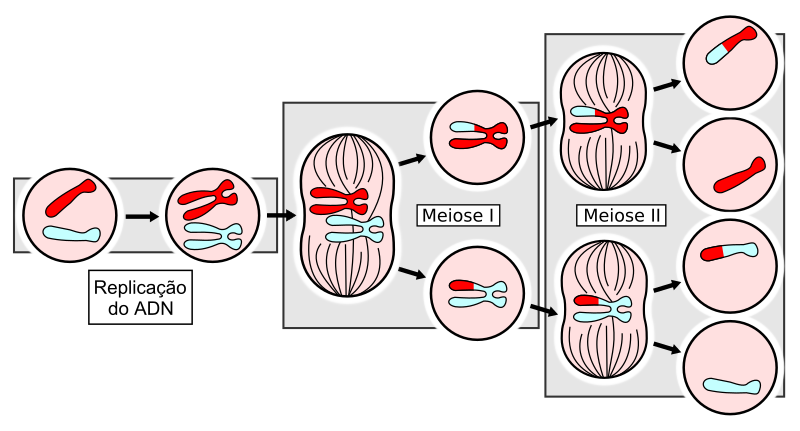
\includegraphics[width=0.4\textwidth]{imagens/meiose.png}
 \caption{Processo de meiose}
 \label{fig:meiose1}
\end{figure}

	
\section{Seleçâo natural moderna e genética de populações}

Agora com todos os conceitos presentados, podemos compreender melhor a seleção natural, desde um ponto de vista mais amplo. A seleção natural trata sobre como certos genes quando expressos em um organismo, podem conferir vantagens adaptativas, tornando esse organismo mais apto a sobreviver e reproduzir-se o que gradualmente formará, ou não, uma nova espécie com o acúmulo de genes distintivos. 

Sendo assim, que acontece quando uma população entra em contato com outra? Ocorre fluxo gênico, ou seja troca de genes de indivíduos de diferentes grupos, e se essa população sofrer deriva genetica modificando cadeias de DNA insignificantes aleatoriamente? na final o fundo genetico da população mudou, sofrendo pequenas variações que a curto prazo não se manifestam, mas ao longo prazo, alteram a espécie tornando-a completamente diferente ao estado inicial.
 
\section{Seleçâo artificial}

A seleção artificial é um processo no qual os seres humanos escolhem características úteis em organismos vivos, como plantas ou animais, para aumentar essas características nas gerações seguintes. Este conceito é aplicado na agricultura, biotecnologia e criado de gados. \\

O procedimento é realizado com a finalidade de obter um recurso, seja um animal de estimação, plantas mais produtivas e resistentes ou gado mais rentável. No momento, é possível notar casos de seleção artificial, como o desenvolvimento de plantas geneticamente modificadas, como soja e milho, e a reprodução seletiva de espécies animais com traços específicos. Em agricultura, são colhidas sementes de plantas mais fortes para obter colheitas melhores e mais saudáveis. Da mesma forma, na pecuária, animais mais férteis ou com melhor carcaça são preferidos, seja na reprodução de gado bovino superior. \\

Neste último ponto, há também a manipulação de engenharia genética, que permite a modificação do DNA de organismos vivos, resultando em plantas ou animais de características avanzadas, contribuindo para a saúde humana, como fabricação de remédios e vacina. O uso da seleção artificial gera debates éticos devido aos possíveis efeitos na diversidade biológica e no bem-estar dos animais.  

\chapter{Evidências Fósseis e Morfológicas da Evolução}\label{chap.Evidencias}

\section{Introdução e Importância de evidências fósseis e morfológicas}\label{sec.fosseis1}

\subsection{Importância de evidências fisícas para a teoria como um todo}\label{subsec.fosseis1.1}

As evidências apresentadas seguem as bases de \cite{prothero2017evolution}, no qual nos baseamos. Como discutido em capítulos anteriores, a seleção natural \ref{sec.selecaon} é o principal motor desse processo, favorecendo as variações benéficas que tornam os organismos mais aptos a sobreviver e se reproduzir.\\

Entre as diversas linhas de evidências que sustentam a teoria evolutiva, as evidências morfológicas e fósseis se destacam como particularmente convincentes. Essas evidências são cruciais para a compreensão da história da vida na Terra, pois fornecem dados concretos e observáveis que permitem traçar as transformações das espécies ao longo das eras geológicas. Além disso, as evidências morfológicas e fósseis não apenas colaboram com a ideia de que a evolução é um processo lento e gradativo, mas também apresentam uma base empírica que torna a teoria do evolucionismo mais difícil de ser refutada. Diferentemente de conceitos mais abstratos, que podem ser mais difíceis de se verificar diretamente.\\

\subsection{Formas as quais são utilizadas essas evidências na prática}\label{subsec.fosseis1.2}

As observações de fósseis e a análise comparativa das estruturas morfológicas de diferentes organismos oferecem uma documentação direta dos vestígios de vida e de sua evolução. O estudo desses elementos possibilita não só a reconstrução das linhagens ancestrais, mas também a identificação de padrões evolutivos que se repetem ao longo do tempo, oferecendo um forte respaldo para a ideia de que as espécies modernas são, de fato, descendentes de formas de vida mais antigas, modificadas ao longo de milhões de anos.\\

Em conjunto, as evidências morfológicas e fósseis formam a espinha dorsal de nossa compreensão do processo evolutivo, proporcionando uma visão palpável e consistente dos mecanismos que moldaram a biodiversidade ao longo da história da vida na Terra.

\section{Evidências Morfológicas}\label{sec.fosseis2}

\subsection{Morfologia}\label{subsec.fosseis2.1}

As evidências morfológicas são fundamentais para a compreensão da evolução das espécies, pois se baseiam nas características estruturais e funcionais dos organismos. Essas características podem ser observadas tanto em espécies atuais quanto em fósseis, e a comparação entre elas oferece descobertas valiosas sobre como as espécies evoluíram ao longo do tempo. Em essência, a morfologia estuda a forma e a estrutura dos organismos, e as evidências obtidas por essa abordagem ajudam a revelar padrões de evolução, adaptabilidade e ancestralidade comum. E geralmente estão divididas em odis tipos de estruturas homólogas e análogas.\\

\subsection{Estruturas homólogas}\label{subsec.fosseis2.2}

Uma das principais contribuições das evidências morfológicas para a teoria evolutiva é a identificação de estruturas homólogas. Essas são estruturas anatômicas que, embora desempenhem funções diferentes em organismos distintos, possuem uma origem evolutiva comum, evidênciada pela similaridade em sua estrutura básica. Um exemplo disso são os membros de vertebrados, como os braços humanos, as asas de morcegos e galinhas, as pernas de um cavalo e as nadadeiras de golfinhos e tartarugas. Apesar de suas funções variadas, essas estruturas possuem uma arquitetura óssea similar que pode ser observada na figura \ref{fig:comparacao_vertebrados}, o que indica que esses grupos de animais compartilham um ancestral comum. A comparação entre essas estruturas fornece uma base sólida para a compreensão de como a evolução pode dar origem a diferentes formas e funções a partir de uma estrutura básica comum.\\

%Adicionar imagem de comparação entre vertebrados%
\begin{figure}[H]
  \centering
  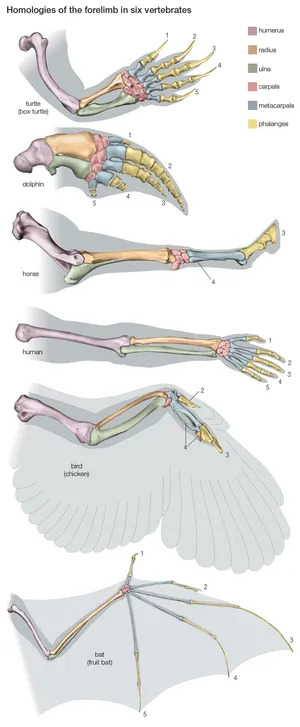
\includegraphics[width=0.5\textwidth]{imagens/ComparacaoVertebrados.jpeg}
  \caption{Comparação entre diferentes vertebrados.}
  \label{fig:comparacao_vertebrados}
\end{figure}

Podemos ver diversas estruturas similares em animais completamente distintos, sendo as estruturas:\\
\begin{itemize}
 \item Úmero 
 \item Rádio
 \item Ulna
 \item Carpo
 \item Metacarpo
 \item Falanges
\end{itemize}

\subsection{Estruturas análogas}\label{subsec.fosseis2.3}

Além das estruturas homólogas, outro conceito importante em morfologia é o das estruturas análogas. Essas são características que, embora desempenhem a mesma função em organismos diferentes, têm origens evolutivas independentes. Um exemplo disso pode ser visto nas asas de insetos e aves. Ambas as estruturas servem para o voo, mas têm origens evolutivas distintas, já que os insetos pertencem a um grupo completamente diferente dos vertebrados. A presença de estruturas análogas pode ser explicada por convergência evolutiva, onde organismos de linhagens diferentes desenvolvem características semelhantes como resultado de adaptações a ambientes ou funções semelhantes, como se mostra em \ref{fig:analogas} .\\

\begin{figure}[H]
  \centering
  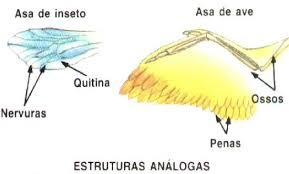
\includegraphics[width=0.5\textwidth]{imagens/aves_e_insetos.jpg}
  \caption{Comparação entre uma asa de um passáro e outra de um inseto.}
  \label{fig:analogas}
\end{figure}

Além disso, o estudo das estruturas vestigiais oferece outra evidência crucial para a teoria da evolução. Estruturas vestigiais são órgãos ou partes do corpo que, ao longo da evolução, perderam a função original que possuíam em espécies ancestrais, o que se pode ver em \ref{fig:baleia}. Um exemplo bem conhecido de estrutura vestigial são os ossos da pelve em cetáceos, como baleias e golfinhos por exemplo. Esses animais, que passaram a viver em ambientes aquáticos, possuem vestígios de membros posteriores, que eram plenamente funcionais em seus ancestrais terrestres, mas se tornaram inúteis para a vida aquática. O fato de essas estruturas ainda estarem presentes nas espécies atuais sugere que as modificações evolutivas são um processo gradual, em que os organismos mantêm vestígios do passado, mesmo que esses atributos tenham perdido sua função adaptativa.\\

\begin{figure}[H]
  \centering
  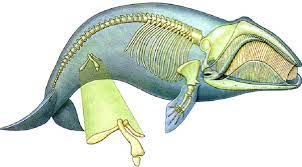
\includegraphics[width=0.5\textwidth]{imagens/baleia.jpeg}
  \caption{Representação de uma Pelve de Baleia}
  \label{fig:baleia}
\end{figure}

\subsection{A Ontogenia}\label{subsec.fosseis2.4}

Indo além dessas evidências, a ontogenia — o estudo do desenvolvimento embrionário dos organismos — também fornece informações morfológicas que colaboram com a teoria evolutiva. O fenômeno conhecido como recapitulação ontogenética, sugerido inicialmente por Ernst Haeckel, propôs que o desenvolvimento embrionário de um organismo reflete, de certa forma, a evolução de sua espécie ao longo do tempo. Embora essa ideia tenha sido revisada, o estudo da ontogenia ainda fornece informações sobre a homologia entre diferentes espécies, pois organismos de diferentes grupos podem passar por estágios de desenvolvimento embrionário similares, o que sugere uma origem comum.\\

\subsection{Métodos de estudo da Ontogenia}\label{subsec.fosseis2.5}

A ontogenia é o estudo do desenvolvimento de um organismo desde a fertilização até a fase adulta,como mencionado anteriormente e há vários métodos utilizados para visualizar embriões de animais e estudar o desenvolvimento embrionário.

\begin{enumerate}
 \item Microscopia de Luz
 \begin{itemize}
  \item \textbf{Microscopia de contraste de fase:} Permite observar células e estruturas internas dos embriões sem a necessidade de corantes. Usada para analisar a morfologia celular e o desenvolvimento inicial sem interferir no processo natural do embrião.
  \item \textbf{Microscopia de fluorescência:} Permite a visualização de estruturas celulares ou moléculas específicas ao usar corantes fluorescentes. Isso é muito útil para identificar proteínas específicas ou processos celulares durante o desenvolvimento, como a migração celular ou a diferenciação de tecidos.
 \end{itemize}
 \item Microscopia Eletrônica (\ac{me})
  \begin{itemize}
   \item \textbf{Microscopia Eletrônica de Varredura \ac{mev}:} Usada para visualizar a superfície do embrião em grande detalhe. Isso pode ser útil para estudar a morfologia externa de embriões de diferentes espécies.
   \item \textbf{Microscopia Eletrônica de Transmissão \ac{met}:} Permite observar detalhes ultraestruturais dentro das células do embrião, como organelas e outras estruturas subcelulares. Essa técnica é mais invasiva e requer cortes finos, mas proporciona informações detalhadas sobre os processos celulares em uma escala nanométrica.
  \end{itemize}
 \item Injeção de Marcadores Fluorescentes
  \begin{itemize}
   \item A \textbf{Injeção de marcadores fluorescentes} em embriões é uma técnica comum para rastrear células específicas ou padrões de desenvolvimento. Um marcador fluorescente (como \ac{gfp}, proteína fluorescente verde) é injetado ou introduzido em células ou tecidos de interesse, representação visual na imagem \ref{fluor}.
   \begin{figure}[H]
   \centering
   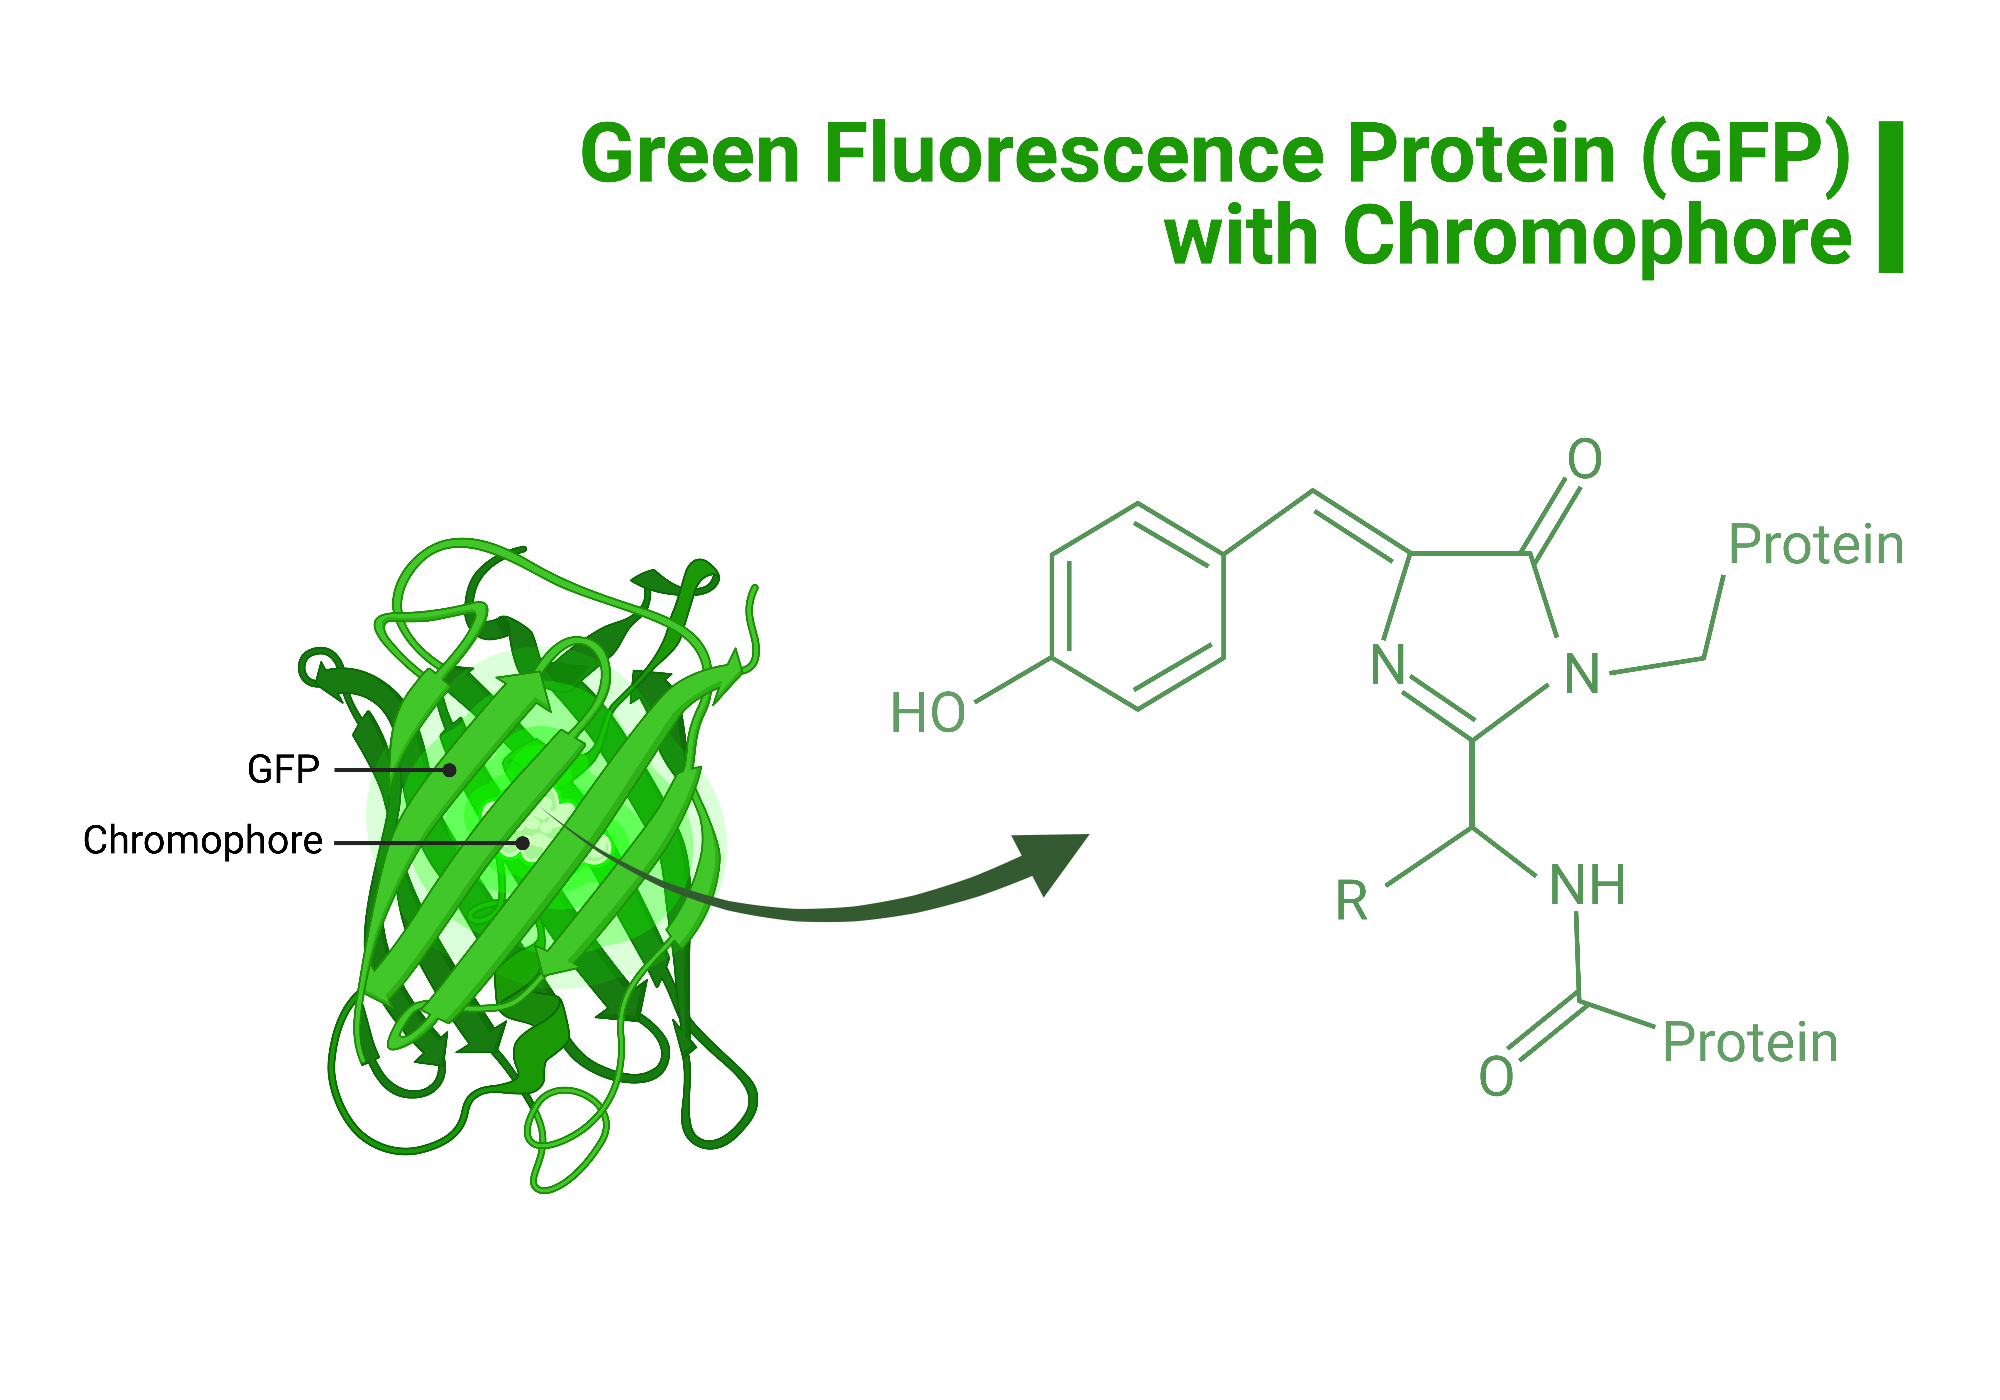
\includegraphics[width=0.5\textwidth]{imagens/gfp.png}
   \caption{Representação de \ac{gfp}}
   \label{fluor}
   \end{figure}
  \end{itemize}
\end{enumerate}

\subsection{Morfologia Molecular}\label{subsec.fosseis2.6}

Por fim, a morfologia comparada também se estende ao nível das estruturas moleculares, como proteínas e DNA. Embora os estudos moleculares sejam frequentemente abordados separadamente da morfologia tradicional, as evidências moleculares também podem ser vistas como uma extensão das evidências morfológicas. Por exemplo, a sequência de aminoácidos em proteínas ou o código genético pode revelar similaridades morfológicas em nível molecular, fornecendo mais uma camada de evidência que sustenta a teoria da evolução.\\

Um exemplo sendo o estudo das estruturas de proteínas e suas funções em Embriões e em seu desenvolvimento, podemos ter como exemplo o \textbf{Citoesqueleto}, que consiste em uma rede de fibras proteicas dentro da célula que proporciona suporte e estrutura, além de ser fundamental para a migração celular. Durante o desenvolvimento embrionário, o citoesqueleto ajuda as células a se moverem para locais específicos, o que é crucial para a formação de tecidos e órgãos.

\subsection{Conclusão sobre Morfologia}\label{subsec.fosseis2.7}

Em suma, as evidências morfológicas são um dos pilares mais sólidos que sustentam a teoria da evolução das espécies. Elas demonstram, de maneira concreta e observável, que as espécies não surgiram de forma independente e imutável, mas sim que elas são modificações de formas de vida anteriores, adaptadas às condições de seus ambientes ao longo do tempo. O estudo da morfologia, desde a comparação de estruturas anatômicas até a análise de componentes moleculares, proporciona uma compreensão profunda de como a evolução moldou a diversidade da vida na Terra, reforçando a ideia de ancestralidade comum e o processo gradual de mudanças ao longo de milhões de anos.\\

\section{Evidências Fósseis}\label{sec.fosseis3}

Os fósseis desempenham um papel fundamental nas descobertas científicas relacionadas à teoria da evolução, funcionando como peças de um "quebra-cabeça" que nos ajudam a entender melhor o desenvolvimento de certas espécies, de forma similiar a qual foi descoberta a separação da Pangeia. O registro fóssil fornece um olhar para o passado da vida na Terra, mostrando como as espécies mudaram ao longo do tempo e como os organismos modernos estão relacionados com formas antigas. Ao longo da história, vários fósseis encontrados desempenharam papéis cruciais no fortalecimento da teoria evolucionista. Hoje em dia conhecemos literalmente milhares de fósseis que mostram a evolução entre os diversos grupos de organismos. Centenas de fósseis demonstram a origem dos mamíferos a partir de sinapsídeos mais primitivos, dos anfíbios a partir dos osteiíctios, a origem dos cetáceos a partir dos mesonquídeos, dos primatas a partir
dos plesiadaptiformes, dos dinossauros a partir de répteis semelhantes a
tecodontes, e da maioria dos principais grupos de vertebrados.

\subsection{Fósseis de transição}\label{subsec.fosseis3.1}

Um \textbf{fóssil de transição} é um tipo de fóssil que exibe características intermediárias entre dois grupos de organismos diferentes, geralmente entre uma espécie ancestral e seus descendentes evolutivamente mais avançados. Esses fósseis são de grande importância para a teoria da evolução, pois fornecem evidências diretas de como as espécies podem ter mudado ao longo do tempo, demonstrando o processo de transformação gradual que Darwin propôs. \\

Esses fósseis mostram uma mistura de traços de grupos distintos, evidenciando estágios intermediários da evolução de uma espécie.

\subsection{O Archaeopteryx}\label{subsec.fosseis3.2}

Um dos fósseis mais famosos que ajudou a reforçar a teoria de Darwin foi o Archaeopteryx, descoberto na Alemanha em 1861. Nas palavras do especialista em aves fósseis J. H. Ostrom (1976) "Possivelmente nenhum outro espécime zoológico, fóssil ou recente, seja considerado tão importante como o Archaeopteryx." Não lhe faltam razões para isso, pois não somente foi o milagroso fóssil que deu certa credibilidade à teoria da evolução proposta por Darwin, como também, tem sido objeto de diversos estudos, provavelmente como nenhum outro fóssil tenha sido antes. 


\chapter{A Evolução nas Espécies Contemporâneas}\label{chap.Evolucao}

A evolução em espécies comtemporâneas da-se pelos fatores já mencionados em capítulos anteriores, como a seleção natural, a variabilidade genética,etc. E támbem vimos que é possível através da analíse fósseis e estruturas morfológicas de animais antigos, descobrirmos diversas informações sobre como decorreu, quanto tempo e por quais fatores houve a evolução de dada espécie para a direção que tomou. Mas agora nese capítulo veremos que também é possível encontrar dados únicos e inovadores em espécies modernas e como elas podem evoluir futuramente.

\section{Experimento com moscas da fruta (Drosophila melanogaster)}\label{sec.cont1}

\subsection{Porque estes animais ?}\label{subsec.cont1.1}

As Drosophila melanogaster (ou moscas-da-fruta como são vulgarmente \ref{Mosca}) são utilizadas para diversos experimentos relacionados com genética e evolucionismo, a curta vida destes insetos, de apenas 10 a 14 dias, dá aos cientistas a oportunidade de estudar múltiplas gerações num curto período de tempo, tornando mais fácil observar como evoluem e transmitem os seus genes. Além disso, essas moscas têm muitos descendentes, o que significa que podemos estudá-las detalhadamente e aprender muito com seu comportamento.\\ 
Também é fácil de cultivar em laboratório, o que o torna uma escolha popular entre os cientistas. As moscas-da-frutas podem ser mantidas em grandes grupos em recipientes especiais, como potes cheios de determinados alimentos, o que torna a realização de experimentos fácil e barata. Além disso, a drosófila tem sido amplamente estudada e podemos ver facilmente suas características físicas, como a cor dos olhos (vermelhos ou brancos), o tamanho do corpo e o formato das asas. Isto permite-nos explorar como as características são transmitidas de pais para filhos e como novas características podem surgir através de mudanças no ADN.\\
Essas vantagens (ciclo de vida curto, fácil manipulação, alta taxa de reprodução e genética bem compreendida) fizeram da Drosophila melanogaster um modelo crucial para o estudo da genética, evolução e seleção natural. É como a espinha dorsal da pesquisa genética, ajudando os cientistas a compreender como as características são transmitidas de uma geração para a seguinte.

\begin{figure}[H]
 \centering
 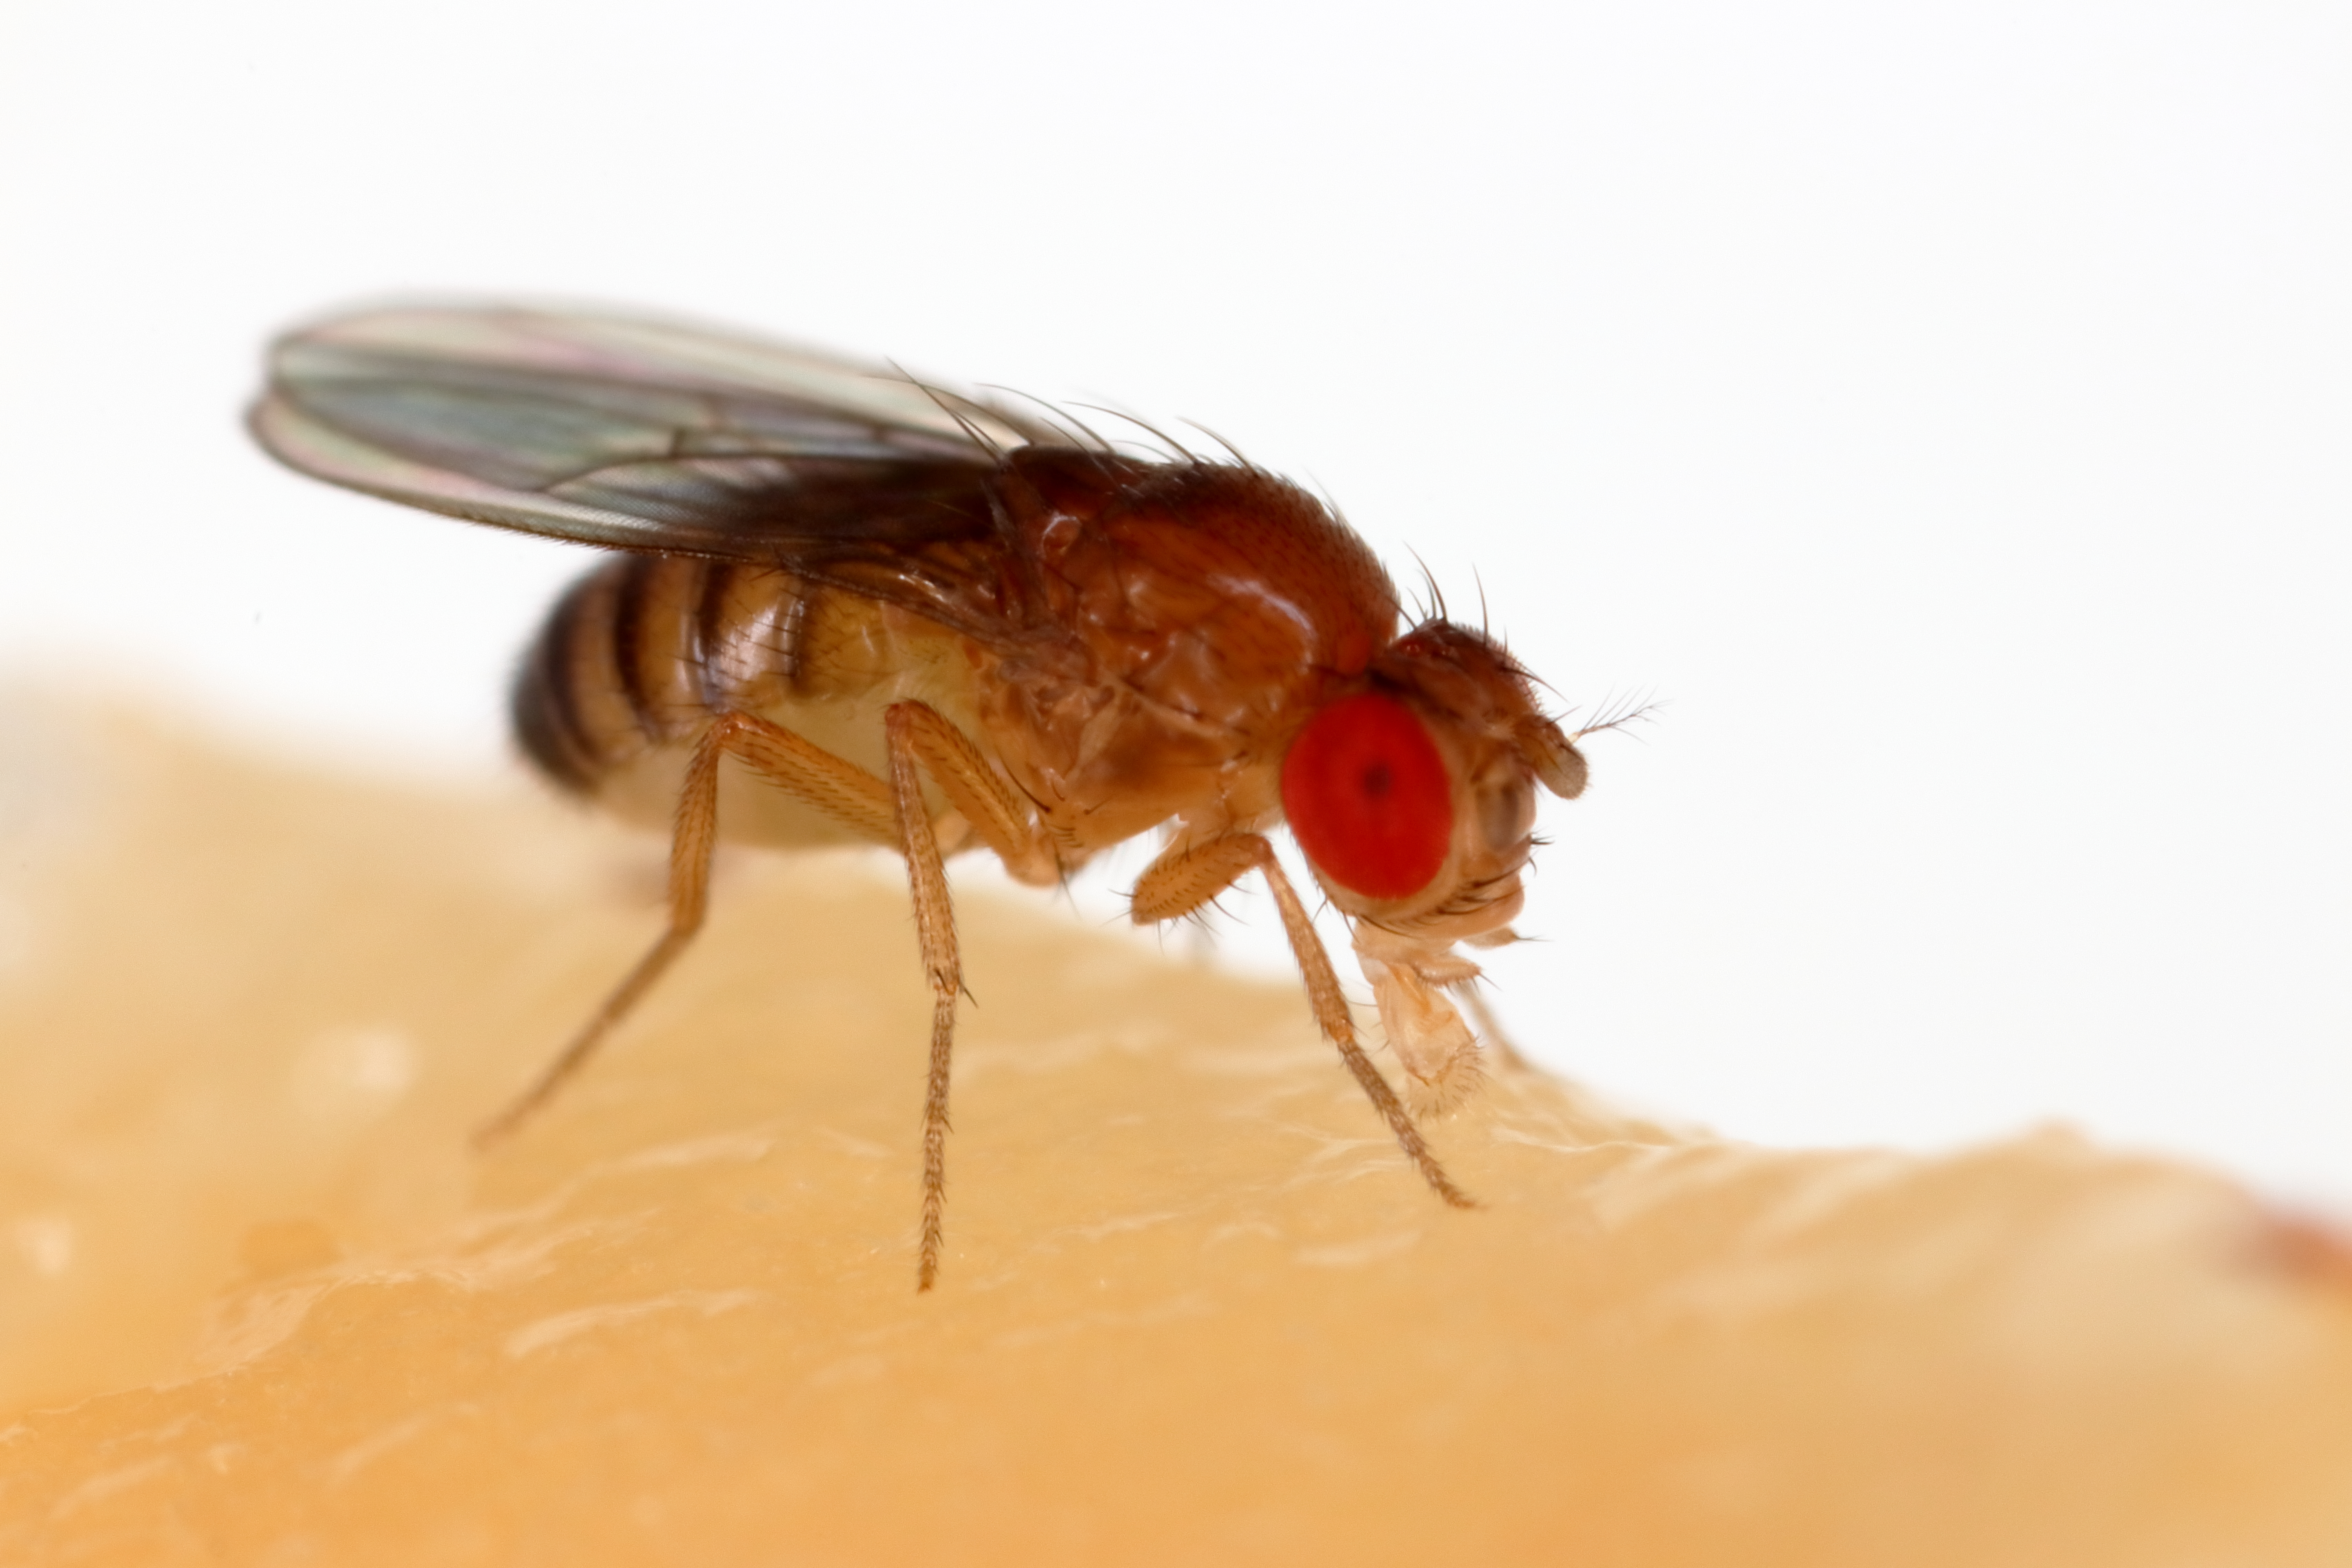
\includegraphics[width=0.5\textwidth]{imagens/Mosca.jpg}
 \caption{Foto real de uma Drosophila melanogaster}
 \label{Mosca}
\end{figure}

\subsection{O Experimento de Seleção Artificial com Drosophilas}\label{subsec.cont1.2}

\subsubsection{Seleção Artificial e Transmissão de Características}\label{subsubsec.cont1.2.1}

Os pesquisadores queriam ver se conseguiriam fazer com que as moscas mudassem as suas características, escolhendo quais gostariam de transmitir aos seus descendentes. As moscas podem não ter características sofisticadas, mas possuem algumas características notáveis, como cor dos olhos, tamanho do corpo ou formato das asas, que podem ser escolhidas. O experimento é muito fácil de controlar porque tudo é muito previsível.
Um exemplo clássico de experimento com drosófila foi o estudo da seleção da cor dos olhos. As moscas podem ter olhos vermelhos ou brancos, dependendo da sua composição genética. Os cientistas tinham o poder de escolher moscas com olhos vermelhos ou brancos para terem descendentes, o que tornou as moscas de olhos vermelhos mais comuns nas gerações subsequentes.

\subsubsection{Seleção de Características Específicas}\label{subsubsec.cont1.2.2}

Os pesquisadores podiam selecionar moscas para determinadas características e acompanhar como essas características se manifestavam nas gerações seguintes. Esse processo permitiu aos cientistas visualizar como a seleção artificial atua na evolução de características fenotípicas.\\

\textbf{Exemplo de seleção de cor dos olhos:}\\

\begin{itemize}
 \item Em um experimento de seleção de cor dos olhos, moscas com olhos brancos (mutação recessiva) seriam    selecionadas para cruzamento, enquanto as moscas com olhos vermelhos seriam descartadas.
 \item Ao longo de várias gerações, a população de moscas teria uma maior frequência de indivíduos com olhos brancos, mostrando como a seleção artificial pode rapidamente mudar as frequências genéticas dentro de uma população.
\end{itemize}

\subsubsection{Seleção de Características Quantitativas}\label{subsubsec.cont1.2.3}

Além das características simples e discretas (como cor dos olhos), a seleção artificial também pode ser aplicada a características quantitativas, que variam em uma escala, como \textbf{tamanho do corpo, duração de vida ou resistência a doenças}.\\
Exemplo: Cientistas podem escolher moscas com um corpo maior para cruzamento. Ao longo de várias gerações, isso levaria a um aumento no tamanho médio das moscas na população. Esse tipo de experimento pode ser usado para estudar a herança poligênica, ou seja, como várias genes interagem para afetar uma característica quantitativa.

\subsubsection{Seleção de Comportamentos}\label{subsubsec.cont1.2.4}

Os experimentos de seleção artificial também podem focar em características comportamentais. Um exemplo famoso de experimento de seleção comportamental foi o de seleção de resistência ao \textbf{estresse}.\\

\begin{itemize}
 \item Seleção de resistência ao estresse: As moscas poderiam ser expostas a condições de estresse (como temperaturas extremas) e as moscas que sobrevivessem a essas condições seriam escolhidas para reprodução. Isso ajudaria a observar como a seleção artificial pode influenciar a \textbf{adaptação comportamental} ao ambiente.
\end{itemize}

\subsubsection{Seleção de Resistência a Drogas ou Químicos}\label{subsubsec.cont1.2.5}

Outro experimento clássico é a \textbf{seleção de resistência a pesticidas}. Em laboratórios, cientistas expuseram as moscas da fruta a \textbf{pesticidas} ou toxinas específicas, e apenas as moscas que possuíssem resistência a essas substâncias conseguiam sobreviver e se reproduzir. Esse processo de seleção artificial ajudou a entender como as populações podem evoluir rapidamente em resposta a pressões seletivas humanas.

\subsection{Conclusões}\label{subsec.cont1.3}

Os experimentos de \textbf{seleção artificial} com \textbf{Drosophila melanogaster} ajudaram a ilustrar como a evolução funciona em um nível genético, confirmando muitas ideias fundamentais da biologia evolutiva, como a herança mendeliana, o papel das mutações e a seleção natural. Além disso, esses estudos forneceram insights importantes sobre como as populações evoluem em resposta a pressões seletivas, incluindo intervenções humanas, e como características podem ser rapidamente selecionadas em uma população.\\
Esses experimentos continuam sendo fundamentais para entender a dinâmica genética das populações e a evolução de características específicas, oferecendo uma base para pesquisas em genética, evolução e até biotecnologia.


\chapter*{Contribuições dos autores}
Os capítulos 2 e 3 foram realizados por \ac{gg} \ quem também foi responsavél da compatibilidade de versões no githhub, enquanto os capítulos 4 e 5 foram realizados por \ac{ht} \ quem também foi responsavél da revisão final, tendo os dois participação ativa na realização do trabalho.

\vspace{10pt}
Percentagem de contribuição de cada autor: \ac{gg} 50\%, \ac{ht} 50\%\\

\vspace{10pt}
\textbf{Repositório GitHub:} \repo

%%%%%%%%%%%%%%%%%%%%%%%%%%%%%%%%%º

\chapter*{Acrónimos}

\begin{acronym}

\acro{gg}[GG]{Gabriel Guzman}
\acro{ht}[HT]{Henrique Tardelli}
\acro{me}[ME]{Microscopia Eletrônica}
\acro{mev}[MEV]{Microscopia Eletrônica de Varredura}
\acro{met}[MET]{Microscopia Eletrônica de Transmissão}
\acro{gfp}[GFP]{Proteína verde fluorescente}

\end{acronym}


%%%%%%%%%%%%%%%%%%%%%%%%%%%%%%%%%

\printbibliography

\end{document}
